\section{Grafi di test}
Dopo l'implementazione degli algoritmi descritta nel capitolo 4, è stato fatto un test con alcuni grafi arbitrariamente costruiti. Come prima cosa, vengono generati manualmente 4 grafi che rappresentano alcuni degli schemi di catene che potrebbero verificarsi all'interno del tx-graph.

Il primo schema rappresenta il classico cammino dritto, e si può notare in figura \ref{fig:straightgraph}
\begin{figure}[htbp]
	\centering
	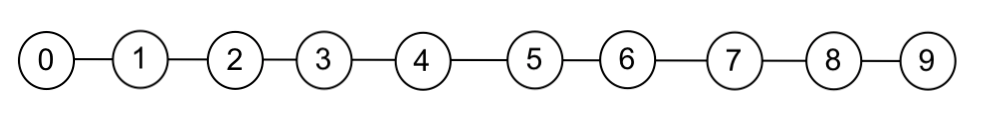
\includegraphics[width = \linewidth]{figure/straightgraph}
	\caption{\textit{Un cammino}\label{fig:straightgraph}}
\end{figure}


Nella figura \ref{fig:ygraph} si può notare un grafo a forma di Y, ovvero due cammini che convergono sullo stesso nodo. Potrebbe essere un classico esempio di una situazione di "merge".
\begin{figure}[htbp]
	\centering
	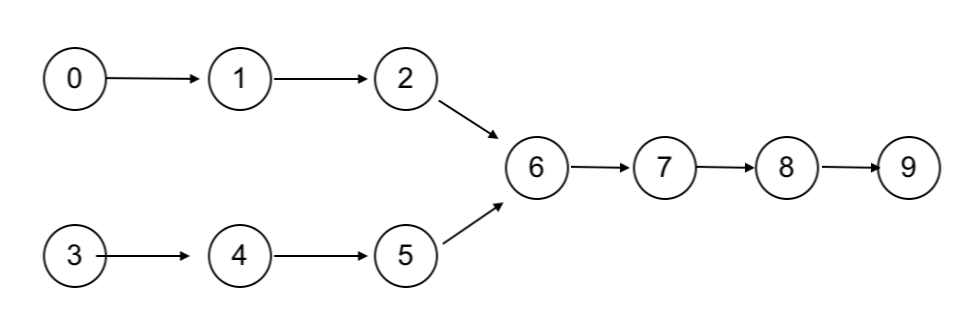
\includegraphics[width = \linewidth]{figure/ygraph}
	\caption{\textit{Un Y grafo}\label{fig:ygraph}}
\end{figure}
%valori attesi
%risultati
\section{MatPlotLib per i grafici}
\section{Statistiche \& Grafici}
\subsection{Al variare di p}
\subsection{Al variare del Dataset}
%istogrammi